\section{Theorie}
\label{sec:Theorie}

\subsection{Fehlerrechnung}

Für die Fehlerfortpflanzung bei Gleichungen mit $N$ fehlerbehafteten Größen
wird jeweils die Formel zur Gaußschen Fehlerfortpflanzung

\begin{equation*}
  \sigma = \sqrt{\sum_{i=1}^{N}\biggl(\frac{\partial f(x_{\g{i}})}{\partial x_{\g{i}}}
  \sigma_{\g{i}}\biggr)^2}
\end{equation*}
mit der jeweiligen Funktion $f(x_{\g{i}})$, den Messgrößen $x_{\g{i}}$ und den
zugehörigen Fehlern $\sigma_i$ verwendet.
Zur Berechnung des arithmetischen Mittels von $N$ Messwerten wird jeweils die
Formel

\begin{equation*}
  \bar{x} = \frac{1}{N}\sum_{i=1}^{N}x_{\g{i}}
\end{equation*}
mit den Messwerten $x_i$ benutzt.
Die Standardabweichung des Mittelwerts wird jeweils mit der Gleichung

\begin{equation*}
  \bar{\sigma} = \sqrt{\frac{1}{N-1}\sum_{i=1}^{N}(x_{\g{i}} - \bar{x})^2}
\end{equation*}
mit den $N$ Messwerten $x_i$ berechnet.

\subsection{Einleitung}

Um mit elektromagnetischen Wellen Informationen zu übertragen, ist es nötig,
diese am Ausgangsort zu modulieren und am Empfangsort zu demodulieren. Bei mehreren Verfahren,
die im Folgenden vorgestellt werden, werden zur Modulation und Demodulation Amplitude, Frequenz und oder Phase der
Welle abhängig vom Ausgangssignal manipuiert.

\subsection{Amplitudenmodulation}

Zum im Folgenden vorgestellten Informationsübertrag durch die sogenannte Amplitudenmodulation sowie auch später zur Frequenzmodulation
wird ein Träger und ein Modulationssignal benötigt. Ausgehend von einer hochfrequenten Trägerschwingung
\begin{align}
  U_{\text{T}}(t) = \hat{U}_{\text{T}} \cos{\omega_{\text{T}} t}
  \label{eqn:traegersch}
\end{align}
und einer niederfrequenten Modulationsschwingung
\begin{align}
  U_{\text{M}}(t) = \hat{U}_{\text{M}} \cos{\omega_{\text{M}} t},
  \label{eqn:modulsch}
\end{align}
wobei $\omega$ jeweils die Frequenz und $\hat{U}$ jeweils die Amplitude bezeichnet,
ergibt sich eine amplitudenmodulierte Schwingung
\begin{align}
  U_3 (t) = \hat{U}_{\text{T}} \left( 1 + m \cos{\omega_{\text{M}} t} \right) \cos{\omega_{\text{T}} t}.
  \label{eqn:amplmod1}
\end{align}
Dabei liegt der sogenannte Modulationsgrad
\begin{align}
  m = \gamma \hat{U}_\text{M}
\end{align}
zwischen 0 und 1 und ist durch die Amplitude der Modulationsschwingung bestimmt.
Die amplitudenmodulierte Schwingung ist in Abbildung \ref{fig:amplmodskizze}
schematisch dargestellt.

\begin{figure}
  \centering
  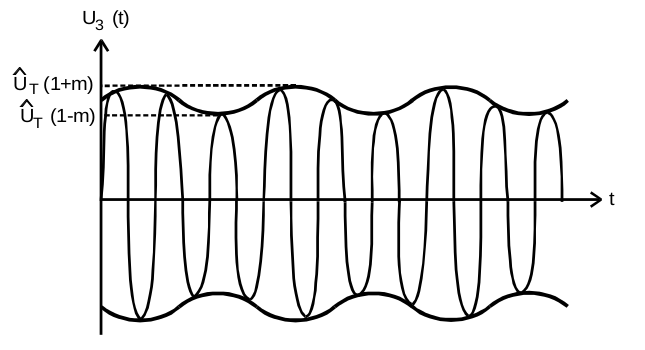
\includegraphics[height=5cm]{JasperErsterSchultag/amplmodskizze.png}
  \caption{Skizze zum Spannungsverlauf der amplitudenmodulierten Schwingung \cite{anleitung}.}
  \label{fig:amplmodskizze}
\end{figure}

Gleichung \eqref{eqn:amplmod1} lässt sich mit Hilfe der Additionstheoreme in einzelne
Kosinuus zerlegen
\begin{align}
  U_3(t) = \hat{U}_\text{T} \cos{\omega_\text{T} t} + \frac12 m \hat{U}_\text{T} \Bigl[ \cos{(\omega_\text{T}+\omega_\text{M}) t} + \cos{(\omega_\text{T}-\omega_\text{M}) t} \Bigr].
\end{align}
Es ergibt sich das in Abbildung \ref{fig:freqspektrum} skizzierte Frequenzspektrum.

\begin{figure}
  \centering
  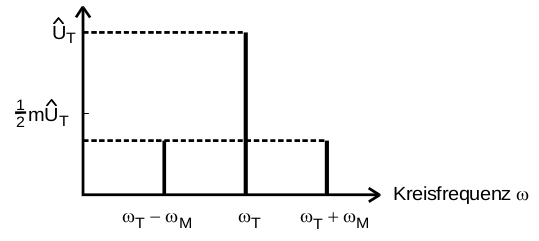
\includegraphics[height=3.5cm]{JasperErsterSchultag/freqspektrum.png}
  \caption{Skizze des Frequenzspektrums einer amplitudenmodulierten Schwingung \cite{anleitung}.}
  \label{fig:freqspektrum}
\end{figure}

Die mittlere Linie beinhaltet ausschließlich die Trägerabstrahlung und beinhaltet keine der zu übertragenden
Informationen. Sie kann und sollte durch spezielle Modulationsverfahren unterdrückt werden, um den Energieverbrauch
zu mindern. Alle Infomationen befinden sich in jeweils beiden Bändern, sodass außerdem im Rahmen einer
Einseitenbandmodulation eines der Bänder, beispielweise mittels eines Bandfilters, abgeschnitten werden kann.
Diverse Nachteile der Amplitudenmodulation, darunter geringe Störsicherheit und Verzerrungsfreiheit, sind
schwieriger zu beheben.

\subsection{Frequenzmodulation}

Bei der sogenannten Frequenzmodulation wird die Amplitude konstant gehalten und eine Frequenzschwingung im Rhytmus
der Modulationsschwingung in eine Trägerschwingung eingebaut. Dies kann mathematisch dargestellt werden durch
\begin{align}
  U(t) = \hat{U} \sin \left( \omega_\text{T} t + m \frac{\omega_\text{T}}{\omega_\text{M}} \cos{ \omega_\text{M} t } \right).
\end{align}
Eine Skizze zu dieser Schwingung ist in Abbildung \ref{fig:freqmodskizze} zu sehen.

\begin{figure}
  \centering
  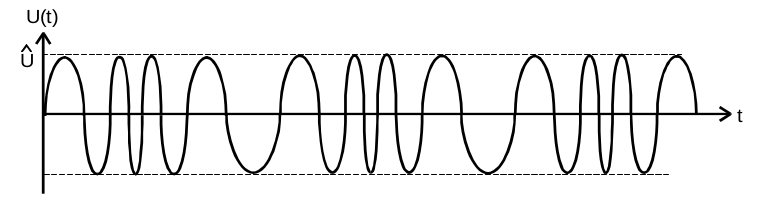
\includegraphics[height=3.5cm]{JasperErsterSchultag/freqmodskizze.png}
  \caption{Skizze zum Spannungsverlauf der frequenzmodulierten Schwingung \cite{anleitung}.}
  \label{fig:freqmodskizze}
\end{figure}

Anstatt einer zeitabhängigen Amplitude ergibt sich eine zeitabhängige Momentanfrequenz
\begin{align}
  f(t) = \frac{w_\text{T}}{2 \pi} (1 - m \sin{\omega_M t}).
  \label{eqn:momentanfreq}
\end{align}
Eine wichtige Kenngröße der Frequenzmodulation ist der sogenannte Frequenzhub
\begin{align}
  f_\text{Hub} = \frac{m w_\text{T}}{2 \pi},
  \label{eqn:frequenzhub}
\end{align}
der die Variationsbreite der Schwingungsfrequenz angibt.
Im folgenden Abschnitt wird die sogenannte Schmalband-Frequenzmodulation vorgestellt,
bei welcher der Frequenzhub klein ist, sodass
\begin{align}
  m \frac{\omega_\text{T}}{\omega_\text{M}} \ll 1.
  \label{eqn:schmalband}
\end{align}
Durch Ausnutzen von Additionstheoremen und einer Taylorentwicklung erster Ordnung, welche
Bedingung \eqref{eqn:schmalband} genügt, ergibt sich die umgeformte, frequenzmodulierte Schwingung
\begin{align}
  U(t) = \hat{U} \cos{\Bigl(\omega_\text{T} t - \frac{\pi}{2}\Bigr)} + \frac12 m \frac{\omega_\text{T}}{\omega_\text{M}}\hat{U}_\text{T} \Bigl[  \cos{(\omega_\text{T}+\omega_\text{M}) t} + \cos{(\omega_\text{T}-\omega_\text{M}) t} \Bigr].
  \label{eqn:freqmod2}
\end{align}
An Gleichung \eqref{eqn:freqmod2} ist erkennbar, dass das Spektrum aus denselben Frequenzen besteht, jedoch
die Phase der Trägerfrequenz $\omega_\text{T}$ um $\frac{\pi}{2}$ phasenverschoben ist.
Die benötigte Taylorentwicklung kann auch bis zu höheren Ordnungen durchgeführt werden, um den Fall einer starken
Frequenzmodulation, also
\begin{align}
  m \omega_\text{T} \approx \omega_\text{M},
\end{align}
abzudecken, das wird in diesem Versuch allerdings nicht benötigt.

\subsection{Schaltungen zur Amplitudenmodulation}
\label{sec:amplmodschaltung}

Um eine Wechselspannung der Form \eqref{eqn:amplmod1} zu erzeugen, werden Bauteile
benötigt, in denen Modulations- und Trägerspannung miteinander multipliziert werden.
Dazu eignen sich diverse Schaltelemente, die eine nichtlineare Spannungskennlinie besitzen,
da durch eine Reihenentwicklung in jedem Fall ein quadratischer Term entsteht, der
unter anderem das Produkt der beiden Spannungen enthält. In diesem Versuch wird unter
anderem der simple Schaltkreis aus Abbildung \ref{fig:primamplmodschaltung} verwendet. Das
nichtlineare Bauteil ist in dieser Schaltung die Diode.

\begin{figure}
  \centering
  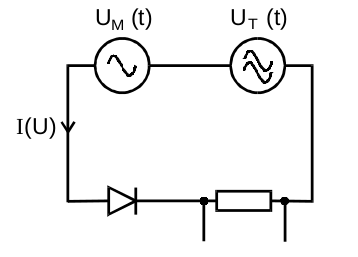
\includegraphics[height=4cm]{JasperErsterSchultag/primamplmodschaltung.png}
  \caption{Skizze eines primitiven Schaltkreises zur Erzeugung einer amplitudenmodulierten Schwingung mittels einer Diode \cite{anleitung}.}
  \label{fig:primamplmodschaltung}
\end{figure}

Problematisch bei der Idee, ein nichtlineares Bauteil einzubauen, um in der Reihenentwicklung
\begin{align}
  I(U_\text{T} + U_\text{M}) = a_0 + a_1 (U_\text{T} + U_\text{M}) + a_2 (U_\text{T}^2 + U_\text{M}^2) + 2 a_2 U_\text{T} U_\text{M} + ...
\end{align}
einen gewünschten Term zu erhalten, ist, dass auch viele Störterme entstehen.
Diese können zwar durch einen Bandfilter unterdrückt werden, da die Frequenzen  weit außerhalb des Bereichs
$[\omega_\text{T} - \omega_\text{M},\omega_\text{T} + \omega_\text{M}]$ liegen, werden aber erzeugt,
weshalb die Schaltung relativ unökonomisch ist.

Ein Schaltelement, das dieses Problem umgeht, ist der sogenannte Ringmodulator, siehe Abbildung \ref{fig:ringamplmodschaltung}.
\begin{figure}
  \centering
  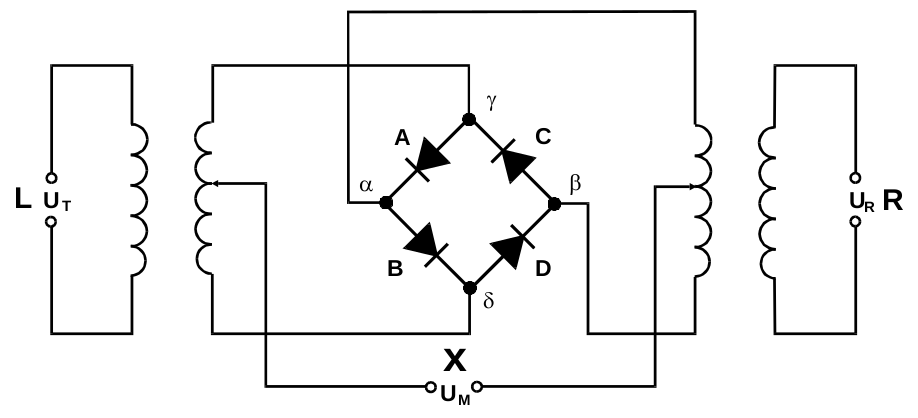
\includegraphics[height=6cm]{JasperErsterSchultag/ringamplmodschaltung.png}
  \caption{Skizze eines Ringmodulators zur Erzeugung einer amplitudenmodulierten Schwingung \cite{anleitung}.}
  \label{fig:ringamplmodschaltung}
\end{figure}
Er besteht aus vier als Ring angeordneten Dioden, die im Idealfall durch das Aufteilen der Eingangsspannungen
eine Spannung mit
\begin{align}
  U_\text{R}(t) = \Gamma U_\text{M}(t) U_\text{T}(t)
\end{align}
am Ausgang R erzeugen, wobei $\Gamma$ eine Konstante ist.
Durch Einsetzen der Trägerschwingung \eqref{eqn:traegersch} und der Modulationsschwingung \eqref{eqn:modulsch} um $\varphi$
phasenverschoben ergibt sich
\begin{align}
  U_\text{R}(t) = \frac{\Gamma}{2} \hat{U}_\text{T} \hat{U}_\text{M} \Bigl[\cos{\bigl((\omega_\text{T}+\omega_\text{M})t + \phi \bigr)} + \cos{\bigl((\omega_\text{T}-\omega_\text{M})t - \phi \bigr)} \Bigr].
\end{align}
Die Trägerabstrahlung wird vollständig unterdrückt und es treten nur zwei Seitenlinien mit Phasenverschiebung auf.

\subsection{Schaltungen zur Frequenzmodulation}

Die im Folgenden vorgestellte Schaltung eignet sich für eine Frequenzmoduation mit geringem Frequenzhub \eqref{eqn:frequenzhub}.
Da, wie in Gleichung \eqref{eqn:freqmod2} erkennbar, zwei amplitudenmodulierte Seitenlinien und eine um $\frac{\pi}{2}$ phasenverschobene Trägerschwingung
benötigt werden, ist es sinnvoll, erneut den Ringmodulator zu nutzen. Zusätzlich wird noch mittels eines Laufzeitkabels am Ausgang die
um $\frac{\pi}{2}$ verschobene Trägerschwingung addiert. Der gesamte Schaltkreis ist in Abbildung \ref{fig:freqmodschaltung} abgebildet.
Um die Leistung der Trägerspannung aufzuteilen und diese später wieder mit der amplitudenmodulierten Spannung zusammenzuführen werden
sogenannte Iso-T's verwendet.

\begin{figure}
  \centering
  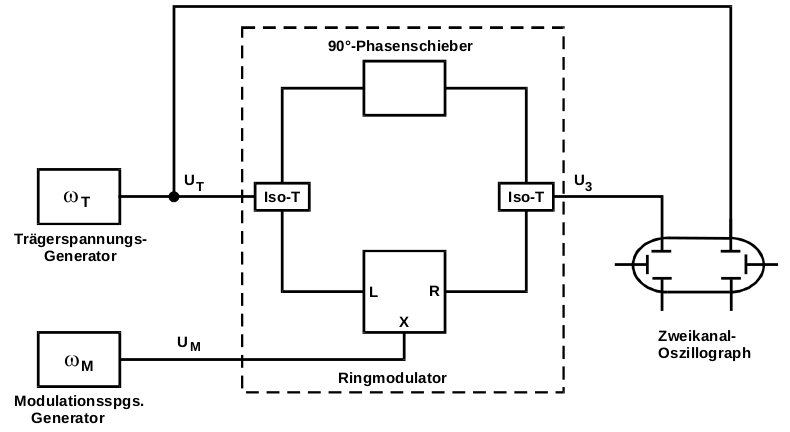
\includegraphics[height=7cm]{JasperErsterSchultag/freqmodschaltung.png}
  \caption{Skizze eines Schaltkreises zur Erzeugung einer frequenzmodulierten Schwingung mittels eines Ringmodulators \cite{anleitung}.}
  \label{fig:freqmodschaltung}
\end{figure}

\subsection{Schaltungen zur Demodulation amplitudenmodulierter Schwingungen}
\label{sec:ampldemod}

Eine durch die Ringmodulatorschaltung modulierte Spannung enthält Schwingungen der
Frequenz $\omega_\text{T}-\omega_\text{M}$ und $\omega_\text{T}+\omega_\text{M}$.
Da ein Ringmodulator bekanntlich die Eingangsfrequenzen addiert bzw. subtrahiert eignet er sich
hier auch zur Demodulation, da er Ausgangsspannungen mit den Frequenzen $\omega_\text{M}$, $2\omega_\text{T} - \omega_\text{M}$ und
$2\omega_\text{T} + \omega_\text{M}$ erzeugt.
Die gesuchte Frequenz kann im Anschluss daran mittels eines Tiefpasses herausgefiltert werden.
Die dazugehörige Schaltung ist in Abbildung \ref{fig:ampldemodschaltung1} zu sehen.
Problematisch ist es unter Umständen, eine phasenstarr mit dem Sender gekoppelte Trägerspannung mit der Frequenz $\omega_\text{T}$
zu erzeugen. Dieses Problem kann mit sogenannten phase-locked-loop-Schaltungen umgangen werden.

\begin{figure}
  \centering
  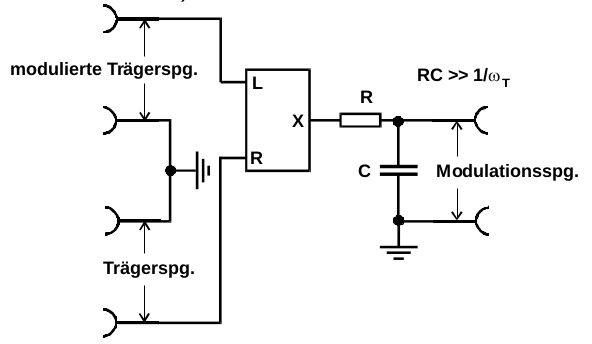
\includegraphics[height=5cm]{JasperErsterSchultag/ampldemodschaltung1.png}
  \caption{Skizze eines Schaltkreises zur Demodulation amplitudenmodulierter Schwingungen mittels eines Ringmodulators \cite{anleitung}.}
  \label{fig:ampldemodschaltung1}
\end{figure}

In Abbildung \ref{fig:ampldemodschaltung2} ist eine Schaltung aufgezeigt, bei der dieses Problem gar nicht erst auftritt.

\begin{figure}
  \centering
  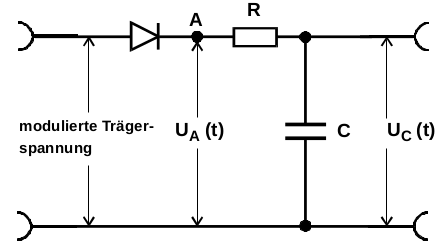
\includegraphics[height=4cm]{JasperErsterSchultag/ampldemodschaltung2.png}
  \caption{Skizze eines Schaltkreises zur Demodulation amplitudenmodulierter Schwingungen mittels einer Diode \cite{anleitung}.}
  \label{fig:ampldemodschaltung2}
\end{figure}

Eine Diode hat die Eigenschaft, dass sie in eine Richtung einen sehr kleinen Widerstand hat und einen Stromfluss zulässt und in die
andere Richtung einen sehr hohen Widerstand hat und quasi isolierend wirkt. Sie kann daher ausgenutzt werden, um in einer amplitudenmodulierten
Wechselspannung, wie sie in Abbildung \ref{fig:amplmodskizze} skizziert ist, die negativen Spannungen abzuschneiden, gemäß der linken Graphik in
Abbildung \ref{fig:diodetiefpass}. Dabei ist zu beachten, dass diese Abbildung idealisiert ist, in der Realität hat die Diode einen zwar geringen, aber
endlichen Durchlass in entgegengesetzte Richtung, sodass ein Streifen mit geringer negativer Spannung nicht abgeschnitten wird.
Desweiteren besitzt die Diode keine lineare Strom-Spannungs-Kennlinie, sodass die Ausgangsspannungen in Durchlassrichtung verzerrt sind.
Für einen geringen Modulationsgrad, wie es in diesem Versuch der Fall ist, ist die Kennlinie
Hinter die Diode ist ein Tiefpass geschaltet, der die Modulationsfrequenz aus der Wechselspannung herausfiltert.

\begin{figure}
  \centering
  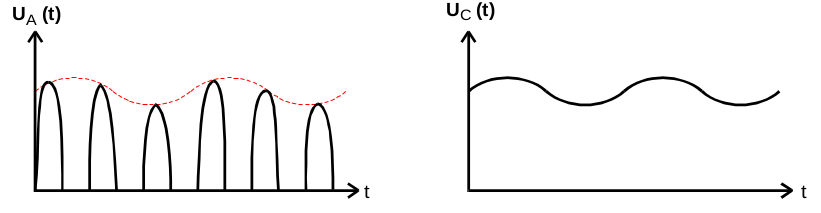
\includegraphics[height=3.5cm]{JasperErsterSchultag/diodetiefpass.png}
  \caption{links: Skizze des Wechselspannungsverlaufs, nachdem die negativen Halbwellen von der Diode abgeschnitten wurden \cite{anleitung}.
  rechts: Skizze des Wechselspannungsverlaufs nach dem Tiefpass \cite{anleitung}.}
  \label{fig:diodetiefpass}
\end{figure}

\subsection{Schaltungen zur Demodulation frequenzmodulierter Schwingungen}

Der Schaltkreis für den sogenannten Flankenmodulator, der in diesem Versuch verwendet wird,
ist in Abbildung \ref{fig:flankendemodulator} abgebildet.

\begin{figure}
  \centering
  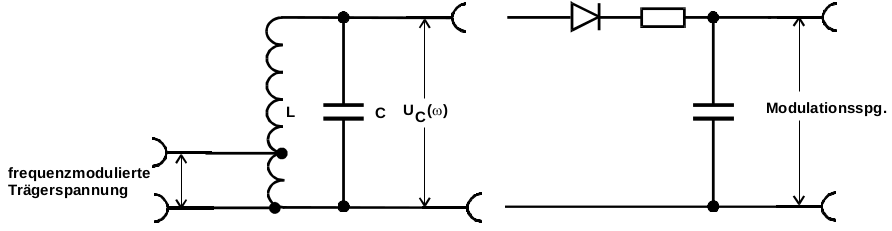
\includegraphics[height=3.5cm]{JasperErsterSchultag/flankendemodulator.png}
  \caption{Schaltkreis des Flankendemodulators zur Demodulation frequenzmodulierter Schwingungen \cite{anleitung}.}
  \label{fig:flankendemodulator}
\end{figure}

Um die frequenzmodulierte Schwingung zu demodulieren
wird diese zunächst in eine amplitudenmodulierte Schwingung umgewandelt und dann mit einer Diode gemäß Abschnitt \ref{sec:ampldemod}
demoduliert. Das Umwandeln in eine amplitudenmodulierte Schwingung ist mittels eines LC-Schwingkreises möglich,
da die Kondensatorspannung im Falle einer erzwungenen Schwingung frequenzabhängig ist. In Abbildung
\ref{fig:freqabh} ist diese Abhängigkeit skizziert. Die Resonanzfrequenz wird so eingestellt, dass die Trägerfrequenz
mitten auf der steilen Flanke der Kurve liegt. Änderungen in der Momentanfrequenz der frequenzmodulierten Schwingung
haben aufgrund der hohen Steigung eine Wechselspannung $U_C(\omega)$ zur Folge, die im Rhytmus der Frequenzmodulation
schwingt. Die Demodulation ist weitestgehend unverzerrt, wenn der Frequenzhub, in Abbildung \ref{fig:freqabh} mit
$\Delta \omega$ bezeichnet, gering ist, da dann die Funktion im Intervall annähernd linear ist.

\begin{figure}
  \centering
  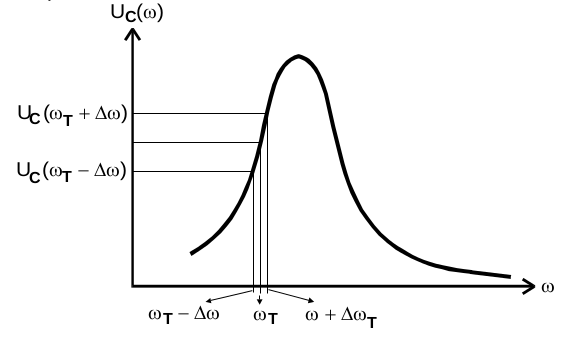
\includegraphics[height=5cm]{JasperErsterSchultag/freqabh.png}
  \caption{Skizze der Resonanzkurve des LC-Schwingkreises \cite{anleitung}. Die Trägerfrequenz sollte zur Optimierung der Demodulation
  wie eingezeichnet mitten auf der steilen Flanke liegen.}
  \label{fig:freqabh}
\end{figure}

\subsection{Bestimmung des Modulationsgrades einer frequenzmodulierten Schwingung}
\label{sec:bestmod}

In Abbildung \ref{fig:bestmod} ist ein beispielhafter Spannungsverlauf einer getriggerten, frequenzmodulierten Schwingung
am Oszilloskop dargestellt.

\begin{figure}
  \centering
  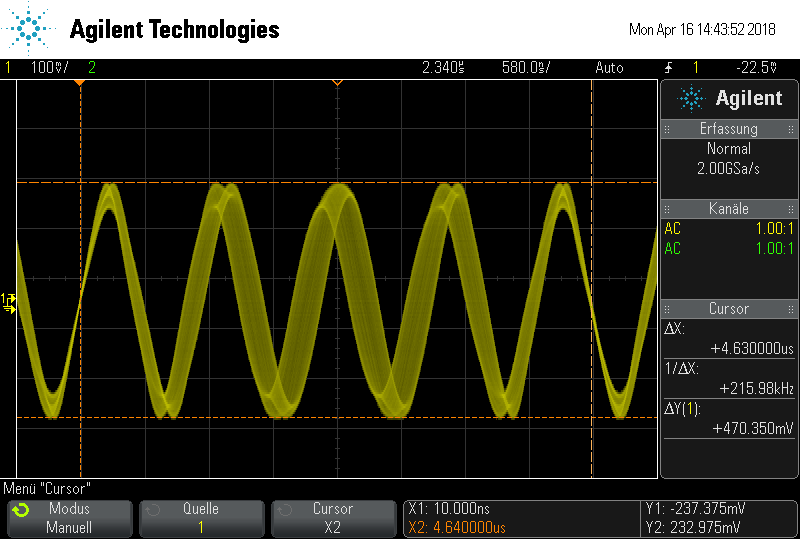
\includegraphics[height=6cm]{Oszi_Pics/freqModRing.png}
  \caption{Beispielhafter am Oszilloskop getriggerter Spannungsverlauf einer frequenzmodulierten Schwingung. Da das Oszilloskop
  nur auf eine feste Spannung triggern kann, entsteht durch Phasenverschiebung ein breiter Streifen.}
  \label{fig:bestmod}
\end{figure}

Die Punkte, an dem der gelbe Streifen minimale Dicke besitzt, sind die
Intervallgrenzen für eine volle Schwingung durch die Modulationsfrequenz. Der Streifen besteht insgesamt aus
einer Funktionenschar an Spannungsverläufen, die sich prinzipiell nur um einen Parameter, die Phasenverschiebung $\varphi$,
unterscheiden. Die Momentanfrequenzen dieser Funktionen werden gemäß Gleichung \eqref{eqn:momentanfreq} beschrieben durch
\begin{align}
  f_{\varphi}(t) = \frac{w_\text{T}}{2 \pi} \bigl(1 - m \sin{(\omega_M t + \varphi)}\bigr).
\end{align}
Durch Integration über die Zeit folgt aus dieser Momentanfrequenz die gesamte Phase, in der sich die frequenzmodulierte
Schwingung befindet. Dies kann ausgenutzt werden, um aus der horizontalen Breite des gelben Streifens aus Abbildung \ref{fig:bestmod}
Rückschlüsse auf den Modulationsgrad der Schwingung zu ziehen. Es ist zweckmäßig, um den Fehler gering zu halten,
die Breite der Linie an der breitesten Stelle abzulesen, sodass sich die beiden Zeitpunkte $t_1 = \frac{\pi}{\omega_\text{M}}$
und $t_2 = \frac{\pi + \delta}{\omega_\text{M}}$ ergeben. Die Spannungskurve zu $t_1$ hat bis zu diesem
Zeitpunkt im Durchschnitt die höchste Frequenz gehabt, da sie ihre Gesamtphase am ehesten erreicht. Die zugehörige Momentanfrequenz
muss also bis zu $t_1$ den größten Integralwert besitzen. Ohne explizite Rechnung ergibt sich, dass die zugehörige
Phasenverschiebung $\varphi_1 = \pi$ ist, da $-m\sin{(\omega_M t + \pi)}$ im Durchschnitt maximal auf diesem Intervall ist.
Analog ergibt sich für $t_2$ die Phasenverschiebung $\varphi_2 = 0$. Die integrierten Frequenzen zu diesen Zeiten und Phasenverschiebungen lauten
\begin{align}
  F_1 = F_{\varphi_1}(t_1) &= \int_{0}^{\frac{\pi}{\omega_\text{M}}} f_{\varphi_1}(t) \symup{d}t \\
  &= \frac{\omega_T}{\omega_M} \left( \frac12 + \frac{m}{\pi} \right) \\
  F_2 = F_{\varphi_2}(t_2) &= \int_{0}^{\frac{\pi+\delta}{\omega_\text{M}}} f_{\varphi_2}(t) \symup{d}t \\
  &= \frac{\omega_T}{\omega_M} \left( \frac{\pi + \delta}{2 \pi} + m(\cos{(\pi + \delta)} - 1) \right).
\end{align}
Da die horizontale Breite vermessen wird, besitzen beide Spannungskurven an den jeweiligen Zeitpunkten dieselbe Gesamtphase $F_1 = F_2$.
Insgesamt ergibt sich daher
\begin{align}
  m = \frac{\delta}{2(1+\pi) + \cos{\delta}},
  \label{eqn:mfuerfreqmod}
\end{align}
wobei
\begin{align}
  \delta = 2 \pi (t_2 - t_1) \omega_\text{M}.
\end{align}
